\chapter{Bend Geometry in Liquid Crystals}
\label{ch:TwistBend}
\begin{figure}[htbp]
    \centering
    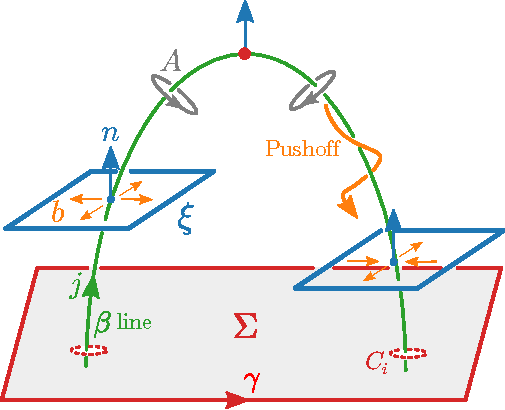
\includegraphics[keepaspectration, width=0.7\linewidth ]{\TwistBendFigures/BetaLine6.pdf}
    \caption{hi}
    \label{fig:BetaLines}
\end{figure}
\section{The structure of bend zeros}

Consider the un-normalised vector field dual to $A$, $\mathbf{B} := \langle b,b \rangle \langle A, \bullet \rangle$ --- the notation $\mathbf{B}$ is chosen to emphasise its similarity to the magnetic field around a current carrying wire. The vector $\mathbf{j} := \nabla \times \mathbf{B}$ points along the $\beta$ lines, orienting them according to the circulation of $A$ and $\mathbf{B}$, as shown in figure~\ref{fig:BetaLines} \cite{MachonThesis}. To see this, consider an orthonormal local trivialisation $(\v d_x, \v d_y,\bf n)$ in a tube around the $\beta$ line. Unlike $(\mathbf{b}, \mathbf{b}_\perp)$, both of which vanish on the $\beta$ line itself, $(\v d_x, \v d_y)$ are perfectly well defined and smooth, although at this stage they are not adapted to the $\beta$ line in any way. In such a trivialisation, ${\bf b} = b_x \v{d}_x + b_y \v{d}_y,\ {\bf b}_\perp = -b_x \v{d}_y + b_y \v{d}_x,\ \langle \v b, \v{b} \rangle = b_x^2 + b_y^2$. Expanding $A$ one finds
\begin{equation}
    A = \frac{b_x d b_y - b_y d b_x}{b_x^2 + b_y^2}+ \omega
    \label{eq:localA}
\end{equation}
where \omega := $\langle \v{d}_y, \nabla \v{d}_x \rangle$ is the connection $1$-form associated to $\nabla$ when using this local trivialisation. $(b_x,b_y,s)$, where $s$ is arclength along the $\beta$ line, form a local coordinate system with assocated unit tangent vectors $(\v{e}_x, \v{e}_y, \v{e}_z) := (\nabla b_x/|\nabla b_x|, \nabla b_y/|\nabla b_y|,\nabla b_x \times \nabla b_y/|\nabla b_x \times \nabla b_y|)$\footnote{We assume that $(b_x, b_y)$ vanish linearly, so $\nabla b_x$ etc. is non-zero on the $\beta$ line and we have a well defined coordinate system.}--- the $z$-axis of this coordinate system lies tangent to the $\beta$ line, but the $\v{e}_x, \v{e}_y$ vectors are currently arbitrary. We may also define the associated cylindrical polar system $(\rho,\theta,z)$, in which $A = d\theta + \omega$; neglecting the smooth $\omega$ component, $A$ circulates as the azimuthal 1-form around the $\beta$ line (figure~\ref{fig:BetaLines}). Multiplying \eqref{eq:localA} through by $b_x^2 + b_y^2$ (which causes the $\omega$ term to vanish on the $\beta$ line) $\v{B} = \frac{e_\theta}{\rho}, \quad \v{j} = \nabla \times \v{B} =\nabla b_x \times \nabla b_y =  \v{e}_z$. We emphasise that, as \eqref{eq:localA} shows, $A$ and $d\theta$ are well defined and continuous along the whole $\beta$ line.

The local structure of a $\beta$ line can be found from a Taylor series or, equivalently, by examining the structure of $\nabla \v b$ on the $\beta$ line --- assuming the $\beta$ line to be generic, $\v b$ vanishes linearly, giving a Taylor series governed by linear terms, with corresponding  non-zero $\nabla \v b$. We  have already seen that the director $\v n$ splits $T \mathbb{R}^3\approx L_n \oplus \xi$, and have used this canonical splitting the break $\nabla \v n$ apart into two pieces , $\nabla_\perp \v n $ and $\nabla_\parallel \v n$ in \S\ref{subsec:Geometry}; we may do the same to $\nabla \v b$. However, the $\beta$ line itself, in combination with $\v n$ along it, actually provides us with more structure --- it gives a canonical way to split $\xi$, giving an adapated framing with which several other splittings may then be defined. In figure \ref{fig:Splittings}(a) we show the $\beta$ line and $\v n$ at a generic point, where $\v n$ and $\v j$ are neither parallel nor perpendicular. The normalised projection of $\v j$ onto $\xi$ defines a new vector $\v n_\chi$, with associated orthogonal plane $\chi$; $\v n \times \v n_\chi$ defines a third vector $\v n_\lambda$ and orthogonal plane $\lambda$. Setting $(\v d_x, \v d_y, \v n) = (\v n_\chi, \v n_\lambda, \v n)$ gives an adapted frame for the $\beta$ line, with the line itself always in the $\lambda$ plane  (note that, as described, this frame is undefined if $\v n \parallel \v j$. Across such points $\v n_\lambda$ changes sign, and as an unoriented plane $\lambda$ may be extended by continuity). We also have the plane perpendicular to $\v j$ itself, given by $\mathrm{ker}(A)$ and spanned by adapted values of $\v e_x,\v e_y$ derived from $\v n_\xi, \v n_\chi$.  
 
Loops in $\mathrm{ker}(A)$, $\xi$ and $\chi$ measure winding in different planes about the $\beta$ line. We have two limiting cases, shown in figures \ref{fig:Splittings}(b) and (c). In figure~\ref{fig:Splittings}(b) $\v  n \parallel \v j$, $\xi = \mathrm{ker}(A)$ and a loop in $\chi$ intersects the $\beta$ line. In figure \ref{fig:Splittings}(c), $\v n \perp \v j$, $\chi = \mathrm{ker}(A)$ and a loop in $\xi$  intersects the $\beta$ line. This latter case, where $\v n \cdot \v j= 0$, we refer to as a Legendrian point \citep{Geiges}.
\begin{figure}[htbp]
    \centering
    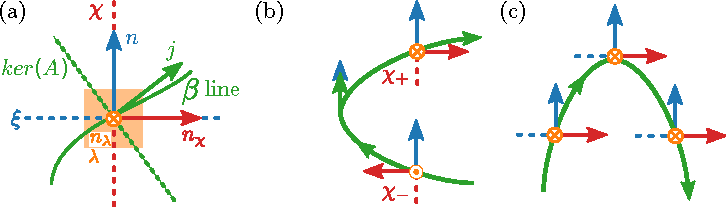
\includegraphics[keepaspectration, width=0.99\linewidth ]{\TwistBendFigures/Splittings.pdf}
    \caption{hi}
    \label{fig:Splittings}
\end{figure}

We now examine the structure of $\nabla \v b$ on the $\beta$ line, making use of the various planes defined above. Note first that, in general, $\nabla \v b \in T^*\mathbb{R}^3 \otimes T\mathbb{R}^3$, however on a $\beta$ line it lies in $T^*\mathbb{R}^3 \otimes \xi$, as $\v n \cdot \nabla \v b = - \v b \cdot \nabla \v n = 0$ on the $\beta$ line.  $\nabla \v b$ has the structure of a linear map $\mathbb{R}^3 \rightarrow \mathbb{R}^2$, with a one-dimensional kernel  which defines the $\beta$ line; $\v j$ lies in this kernel. We have that 
\begin{equation}
\v j = \mathrm{det}(\nabla^{\ker(A)}\v b) \v e_3 = \mathrm{det}(\nabla^\xi \v b) \v n + \mathrm{det}(\nabla^\chi \v b) \v n_\chi
\label{eq:IndexRelation}
\end{equation}
where $\nabla^\chi \v b$, for example, is the restriction of $\nabla \v b \in T^*\mathbb{R}^3 \otimes \xi $ to the space $\chi^* \otimes \xi$ (as a linear map between vector spaces of the same dimension, its determinant is well defined). Each equality in this result is just a rewriting of the cross product $\nabla b_x \times \nabla b_y$, but they may be obtained more directly and transparently by pulling back the volume form on $\xi$ via $\nabla \v b$. Using the second equality  in \eqref{eq:IndexRelation} as an example, we have the decomposition $\nabla \v b = \nabla^\xi \v b + \nabla^\chi \v b $, which carries through to the pullback, and since each of $\nabla^\xi \v b, \nabla^\chi \v b$ are maps between vector spaces of the same dimension, the pullback simply scales the volume form by the determinant. \eqref{eq:IndexRelation} relates the various windings we see in different measuring loops around the $\beta$ line, and allows us to clearly examine winding behaviour as we pass through a Legendrian point. The most common measurement \citep{Nye1987,Berry1998,Berry2004} is $\v n \cdot \v j = \mathrm{det}(\nabla^\xi \v b)$, which describes the winding of $\v b$ measured on a loop in the oriented plane $\xi$ (oriented as dual to $\v n$); its sign has been taken to define an `index' for the $\beta$ line \citep{Nye1987,Berry1998,Berry2004}, which we denote $I^\xi_{\beta} :=  \mathrm{Sgn}(\v{n} \cdot \v{j})$. Analogously one also defines an index $I^\chi_\beta := \mathrm{Sgn}(\v{n_\chi} \cdot \v{j})$, measuring winding on $\chi$. The absence of $I^\lambda_\beta$ is by construction of our framing: $\mathrm{det}(\nabla^\lambda \v b) =0$ identically. Let us now consider what happens as we pass through a Legendrian point. Here, $\v n \cdot \v j =0$, and $\det(\nabla^\xi \v b)$ vanishes. If we measure winding in $\xi$ at this point, we encounter degenerate behaviour. However, the winding measured in $\mathrm{ker}(A) = \chi$, given by $\mathrm{det}(\nabla^\chi \v b)$, is perfectly well behaved --- indeed, in general we have that $\mathrm{det}(\nabla^{\ker(A)}\v b)^2 = \mathrm{det}(\nabla^\xi \v b)^2+ \mathrm{det}(\nabla^\chi \v b)^2$, and so winding in the $\mathrm{ker(A)}$ plane is of constant sign.

Let us explore how all this looks in a concrete co-ordinate system. Suppose we are given a framing $(\v d_x,\v d_y,\v n)$, currently not adapted to the $\beta$ line, with respect to which $\nabla \v b$ is a $2\times3$ matrix and we have a Taylor series
\begin{align}
\begin{pmatrix}b_x \\ b_y\end{pmatrix} = 
\begin{pmatrix} 
    \nabla^\xi \v b_{xx} & \nabla^\xi \v b_{xy} & s_{xz}\\
    \nabla^\xi \v b_{yx} & \nabla^\xi \v b_{yy} & s_{yz}\\ 
\end{pmatrix}
\begin{pmatrix}x \\ y \\ z \end{pmatrix}  
+ O(2)
\label{eq:gradbmatrix}
\end{align}
where $s_{xz},s_{yz}$ are currently regarded simply as undetermined constants in the Taylor series. How should we extract data from this matrix? Firstly, we have that 

\begin{align}
    \v j &= (\nabla^\xi \v b_{xy}s_{yz} - \nabla^\xi \v b_{yy}s_{xz})\v d_x -( \nabla^\xi \v b_{xx}s_{yz} - \nabla^\xi \v b_{yx}s_{xz})\v d_y + \mathrm{det}(\nabla^\xi b) \v n \\
&= \mathrm{det}(\nabla^{\chi^{'}} \v b)\v d_x  -\mathrm{det}(\nabla^{\lambda^{'}} \v b)\v d_y + \mathrm{det}(\nabla^\xi \v b) \v n 
\end{align}
We place primes on $\chi$ and $\lambda$ to as a reminder that these are the planes associated with the currently unadapted frame $(\v d_x,\v d_y, \v n)$. 


%, which tells us to rotate the $x$-$y$ plane, i.e. $\xi$, such that the first and third columns of \eqref{eq:gradbmatrix} are colinear. This done, we compare to \eqref{eq:IndexRelation}.


OLD STUFF OLD STUFF




 We may relate the operators defined above to director derivatives; a direct calculation yields $\nabla^\xi \v{b} = (\nabla^\xi{\bf n}|_{0})^2+\nabla^L \nabla^\xi{\bf n}|_{0}$ , $\nabla^L \v b = (\nabla^L)^2 \v n$. $\nabla^{\xi}{\bf n} \bigr|_{0}$ (with entries $\partial_j n_i$, $i,j=x,y$ with respect to our frame) defines a linear transformation on the plane perpendicular to the director ($xy$-plane), and is called the shape operator of the director field~\cite{machon16,alexander18}. This relevant Taylor series for the director, retaining only terms that contribute to the bend at linear, is
\begin{align}
\begin{pmatrix} n_x \\ n_y \end{pmatrix} & = \biggl( \Bigl. \nabla^\xi {\bf n} \Bigr\rvert_0 + z \Bigl. \bigl( \nabla^L\nabla^\xi {\bf n} \bigr) \Bigr\rvert_0 \biggr) \begin{pmatrix} x \\ y \end{pmatrix} + \frac{1}{2} z^2 \begin{pmatrix} (\nabla^L)^2 n_x \\ (\nabla^L)^2 n_y \end{pmatrix}, \\
\end{align}
giving bend
\begin{align}
\begin{pmatrix}b_x \\ b_y\end{pmatrix} & =
 \biggl( \Big( \Bigl. \nabla^\xi {\bf n} \Bigr\rvert_0 \Big)^2 + \Bigl. \nabla^L\nabla^\xi {\bf n} \Bigr\rvert_0 \biggr) \begin{pmatrix} x \\ y \end{pmatrix}
 + z \begin{pmatrix}(\nabla^L)^2 n_x \\ (\nabla^L)^2 n_y \end{pmatrix}
\label{eq:LocalBend}
\end{align}
which may then be cast into the form of \eqref{eq:LocalBendMatrix}.

$\nabla^\xi \v{b}$ itself may be further decomposed into two components, a spin 0 component $\nabla^{\xi, +} \v{b}$ with positive determinant and winding and a spin 2 component $\nabla^{\xi, -} \v{b}$ with negative determinant and winding: $\nabla^\xi \v{b} = \nabla^{\xi,+} \v{b} + \nabla^{\xi,-} \v{b}$ \cite{MachonThesis}. With this decomposition one finds that $\v{n} \cdot \v{j} = \mathrm{det}(\nabla_\perp \v{b}) = |\mathrm{det}(\nabla_\perp^+ \v{b})| - |\mathrm{det}(\nabla_\perp^- \v{b})|$. Each of these components may be expressed in terms of the director. To do so, we recall the splitting of the shape operator \eqref{eq:GradientDecompositionperp}
\begin{align}
    \nabla^\xi {\bf n}= \frac{\nabla \cdot {\bf n}}{2}I - \frac{{\bf n} \cdot \nabla \times {\bf n}}{2} J + \Delta
\end{align} 
which with respect to our local $(\v d_1,\v d_2,\v n)$ basis reads 
\begin{align}
 \nabla^\xi {\bf n}=\begin{pmatrix} s/2 + \Delta_1 & -q/2 + \Delta_2 \\ q/2 + \Delta_2 & s/2 - \Delta_1 \end{pmatrix} ,
\end{align} 
where $s = \nabla \cdot \v n$ is the splay, $q = \v n \cdot \nabla \times \v n$ is the twist and $\Delta_1$, $\Delta_2$ are the deviatoric components~\cite{machon16,selinger19}. One finds that
\begin{align}
\nabla^{\xi,+} \v{b} &=
\frac{1}{4}\Big(s^2 - q^2 + 4\Delta_1^2 + 4\Delta_2^2 +2\partial_z s\Big)I+
\frac{1}{2} \Big(sq + \partial_z q \Big)J  \\
\nabla^{\xi,-} \v{b} &= s \Delta +\partial_z \Delta 
\end{align}
 Note that in the absence of $z$ variation, $\nabla^\xi \v{b}$ is an exact square and only an index of $I_\beta = +1$ as possible. The potential for negative winding is thus entirely contained within $\partial_z \Delta$. Explicitly, $\v{n} \cdot \v{j} = \mathrm{det}(\nabla^\xi \v{b}) = \left( (s/2)^2 +(q/2)^2 -\Delta_1^2 - \Delta_2^2\right)^2 +\left(s(q/2)^2 + \partial_z (q/2)\right)^2 - (\partial_z \Delta_1) ^2 - (\partial_z \Delta_2)^2 - s \partial_z(\Delta_1^2 + \Delta_2^2)$.  In figure \ref{fig:LocalProfiles} we show a variety of bend zeros with indices $I_\beta = \pm 1$ and their accompanying modes of director distortion.

\begin{figure}[htbp]
    \centering
    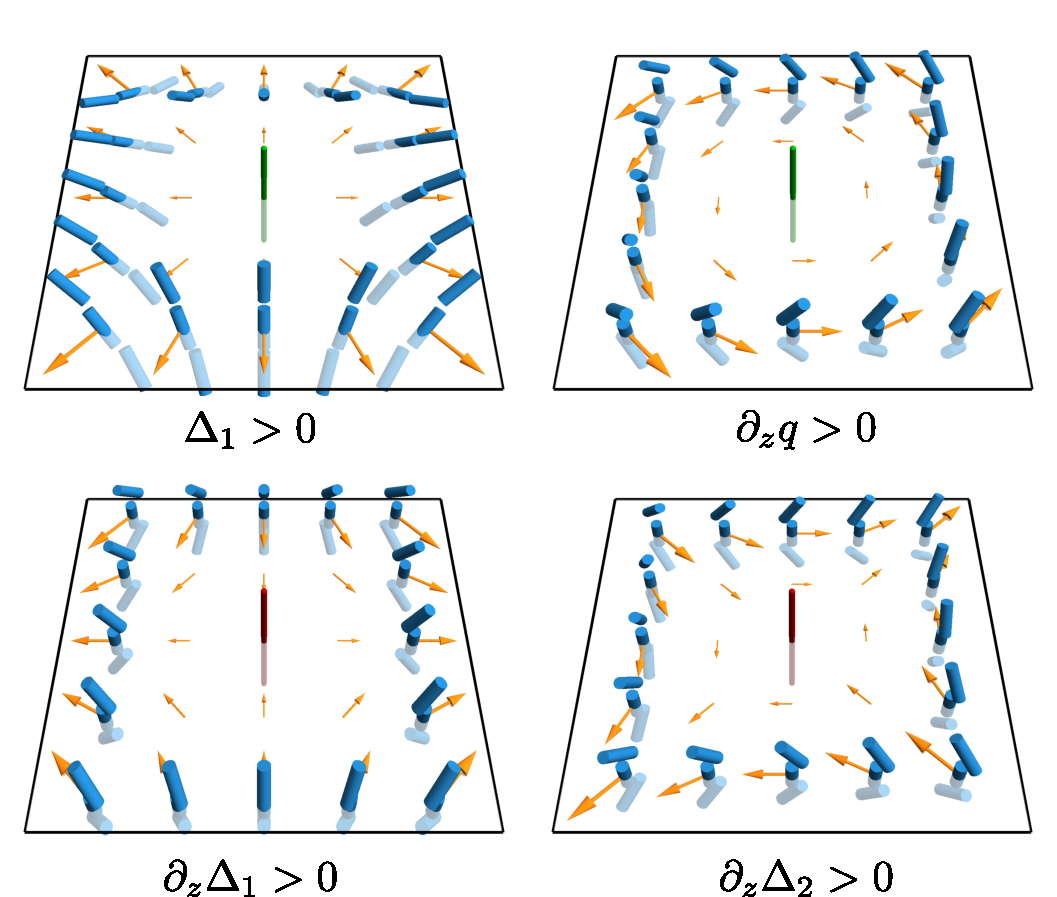
\includegraphics[keepaspectration, width=0.7\linewidth ]{\TwistBendFigures/LocalProfiles.pdf}
    \caption{Local profiles about $I_\beta = +1$ (green line) and $I_\beta = -1$ (red line) bend zeros, with director (blue cylinders) and bend vector (orange) shown in cross-section. Each panel shows the effect of a single parameter in  with the rest set to zero. $z$ variation in $\Delta$ is essential for a $I_\beta = -1$ zero.}
    \label{fig:LocalProfiles}
\end{figure}


The operator $\nabla_\perp \v{b} := (\nabla_{\perp}{\bf n}|_{0})^2+\partial_z \nabla_{\perp}{\bf n}|_{0}$ controls the structure of $\v{b}$ in the plane $\xi$, and the two numbers $s_x:=\partial_{zz} n_x|_0$, $s_y:=\partial_{zz} n_y|_0$ control the skew between the $\beta$ line and the director as explained below. The matrix of orthogonal derivatives $\bigl. \nabla_{\perp}{\bf n} \bigr|_{0}$ (with entries $\partial_j n_i$, $i,j=x,y$) defines a linear transformation on the plane perpendicular to the director ($xy$-plane), and is called the shape operator of the director field~\cite{machon16,alexander18}. From \eqref{eq:LocalBend} one has that $\v j = (\nabla_\perp \v{b}^{\dagger} \v{s}, \mathrm{det}(\nabla_\perp \v b))$, where $\v{s}:=(s_x,s_y)$ and $\dagger$ denotes the matrix adjugate\footnote{The adjugate, defined by the condition that $AA^{\dagger} = A^\dagger A = \mathrm{det}(A)I$, exists even when $\mathrm{det}(A)=0$.}. We see that $\v{n}\cdot \v{j} = \mathrm{det}(\nabla_\perp\v{b})$, and so the index $I_\beta$ is $\pm 1$ according to the sign of $\mathrm{det}(\nabla_\perp \v b)$. Note that Legendrian points are then given by the condition that $\mathrm{det}(\nabla_\perp\v{b})=0$. 

If we are at a transverse point, $\v j$ can also be written as $\v{j} = \mathrm{det}(\nabla_\perp \v b)(\nabla_\perp \v b^{-1}\v{s},1)$, a result which may be arrived at directly by factoring out $\nabla_\perp \v b$ from \eqref{eq:LocalBend}. Here $\nabla_\perp \v b^{-1}\v{s}$ transparently controls the skew between the $\beta$ line and $\bf n$, acting as a homogenous coordinate on the space of lines through the origin, which breaks down when describing a Legendrian $\beta$ line lying in the $xy$-plane.  By contrast, at a Legendrian point $\v j = (\nabla_\perp \v{b}^{\dagger} \v{s},0 )$, and as $\nabla_\perp \v b \nabla_\perp \v{b}^{\dagger} \v{s} = 0$, the orientation of the $\beta$ line in the $xy$-plane is controlled by $\mathrm{ker}(\nabla_\perp \v b)$. This kernel defines a splitting of $\xi \approx \mathrm{ker}(\nabla_\perp \v b) \oplus \mathrm{ker}(\nabla_\perp \v b)^\perp $, and hence an overall splitting $\mathbb{R}^3 \approx \xi_+ \oplus \xi_- \oplus L_n$. The operator $\left[\begin{array}{c|c} \nabla_\perp \v b|_{\mathrm{ker}(\nabla_\perp \v b)^\perp} & \v s \end{array}\right]$ describes the winding of $\v b$ in the plane perpendicular to the $\beta$ line, $\xi_+ \oplus L_n$.


\begin{comment}


 The local structure of a $\beta$ line can be found from a Taylor series or, equivalently, by examining the structure of $\nabla \v b$ on the $\beta$ line --- assuming the $\beta$ line to generic, $\v b$ vanishes linearly, giving a generic Taylor series governed by linear terms, with corresponding  non-zero $\nabla \v b$. We begin by splitting $T\mathbb{R}^3 \approx L_n \oplus \xi$, with corresponding operator splitting $\nabla \v b = \nabla^{L} \v b + \nabla^\xi \v b $, where, for example, $\nabla^L(\bullet) $ is the restriction of $\nabla (\bullet) \in T\mathbb{R}^3 \otimes T\mathbb{R}^3$ to the space $L_{\v n}^* \otimes T\mathbb{R}^3 $. Using $\v n\cdot \v b =0$ one finds that $\nabla^L \v b \in L_n^* \otimes \xi$. In general $ \nabla^{\xi} \v b \in \xi^* \otimes (L_n \oplus \xi)$, however on the $\beta$ line $\v n \cdot \nabla^\xi \v b = -\v b \cdot \nabla^\xi \v n =0$, so we may safely consider $\nabla^{\xi} \v b \in \xi^* \otimes \xi$. In the language of a Taylor expansion $\v b = (b_x,b_y,b_z)$ of director $\v n \approx (n_x,n_y,1)$ in the $(\v d_x,\v d_y,\v d_z = \v n)$ frame about a $\beta$ line, we have that to linear order $b_z=0$ and 
\begin{align}
\begin{pmatrix}b_x \\ b_y\end{pmatrix} & = \left(\begin{array}{c c |c} (\nabla^\xi \v b) _{xx}&(\nabla^\xi \v b) _{xy}& (\nabla^L \v b)_x  \\
 (\nabla^\xi \v b) _{yx}&(\nabla^\xi \v b) _{yy} & (\nabla^L \v b)_y
 \end{array} \right) \begin{pmatrix} x \\ y \\ z \end{pmatrix} 
\label{eq:LocalBendMatrix}
\end{align}
where the vertical line emphasises the splitting at play. One notes immeadiately that, as a linear map $\mathbb{R}^3 \rightarrow \mathbb{R}^2$, $\nabla \v b$ has a one dimensional kernel which defines the $\beta$ line to linear order, and that this kernel is along $\v j= \nabla b_x \times \nabla b_y$, consistent with the above discussion. One also notes that $\v n \cdot \v j = \mathrm{det}(\nabla^\xi \v b)$, a point we shall discuss in greater detail below.





 The latter control the relative orientation between the tangent to the $\beta$ line and the local director, while the former determine the winding number of the zero and also its geometry.


$\pm 1$ according to the sign of $\det\bigl( (\nabla_{\perp}{\bf n}|_{0})^2+\partial_z \nabla_{\perp}{\bf n}|_{0} \bigr)$. When the derivatives $\bigl. \partial_z \nabla_{\perp}{\bf n} \bigr|_{0}$ are negligible this is always $+1$, so that the different profiles of $\beta$ lines are controlled crucially by these parallel derivatives of the shape operator. These split naturally into two contributions


 It describes the splay $s$ and twist $q$ of the director, as well as the directions of principal curvature, and may be written
\begin{equation}
\Bigl. \nabla_{\perp} {\bf n} \Bigr|_{0} = \begin{bmatrix} s/2 + \Delta_1 & -q/2 + \Delta_2 \\ q/2 + \Delta_2 & s/2 - \Delta_1 \end{bmatrix} ,
\end{equation}
where $\Delta_1$, $\Delta_2$ are the deviatoric components~\cite{machon16,selinger19}. The matrix $\bigl. \partial_z \nabla_{\perp}{\bf n} \bigr|_{0}$ describes how these quantities vary as one moves along the director field.

\begin{equation}
\Bigl. \partial_{z} \nabla_{\perp} {\bf n} \Bigr|_{0} = \begin{bmatrix} \partial_z s/2 & -\partial_z q/2 \\ \partial_z q/2 & \partial_z s/2 \end{bmatrix} + \begin{bmatrix} \partial_z \Delta_1 & \partial_z \Delta_2 \\ \partial_z \Delta_2 & -\partial_z \Delta_1 \end{bmatrix} , 
\label{eq:local_windings}
\end{equation}
corresponding to positive and negative winding, respectively. {\sl GPA: more here ...} %thing to do here
The different local profiles of the director, and its bend, around a general point on a $\beta$ line are shown in Fig.~\ref{fig:profiles}.











\section{Topological Significance}

On the complement of the bend zeros, we define an orthonormal connection 1-form
\begin{equation}
    A = \langle \nabla \tilde{e}_1 ,\tilde{e}_2 \rangle = \frac{\langle \nabla e_1 ,e_2 \rangle}{\langle e_1,e_1 \rangle}  
\end{equation}

where $\tilde{e}_i$ is the normalised version of $e_i$. A few remarks about this definition are in order. Firstly, the connecction $\nabla$ at play here is a connection on the bundle $\xi$, and is globally well defined as the restriction of the ambient connection of manifold to the plane field. Equivalently, it is the pullback connection induced by the map ${\bf n}: M \rightarrow S^2$ --- this second formulation is good to remember. The sections $(e_1,e_2)$ are, however, only well defined on the complement of the bend zeros, and this carries through to $A$. 

Inserting a measuring surface $\Sigma$ with boundary $\gamma$ into $M$ one has a Gauss-Bonnet style result:
\begin{equation}
 \int_\gamma A - \int_\Sigma dA = \sum_i \int d \theta = \sum_i \mathrm{index}_\Sigma \beta_i
\end{equation}
The sum of these indices computes the degree of the map ${\bf n}:\Sigma \rightarrow S^2$, known as the skyrmion number. This is analogous to how the integration of the curvature form computes the degree of the Gauss map, and this again may be computed by summing the umbilic points of a surface. The number of $\beta$ lines facilitates this same count.

$A$, considered as a vector field $\bf A$, orients the umbilics , its curl giving a tangent vector, $\bf B = \nabla \times \bf A$. Thinking in terms of the magnetostatic potential and field around a wire, this is not overly surprising. One should weight the local profile around a $\beta$ line by the factor $\mathrm{Sgn}(\bf n \cdot B)$. The switches signs when the $\beta$ line is not transverse to the plane field $\xi$.


\end{comment}
